\documentclass[tikz,border=2mm]{standalone}
\usetikzlibrary{arrows.meta, decorations.pathreplacing}

\begin{document}
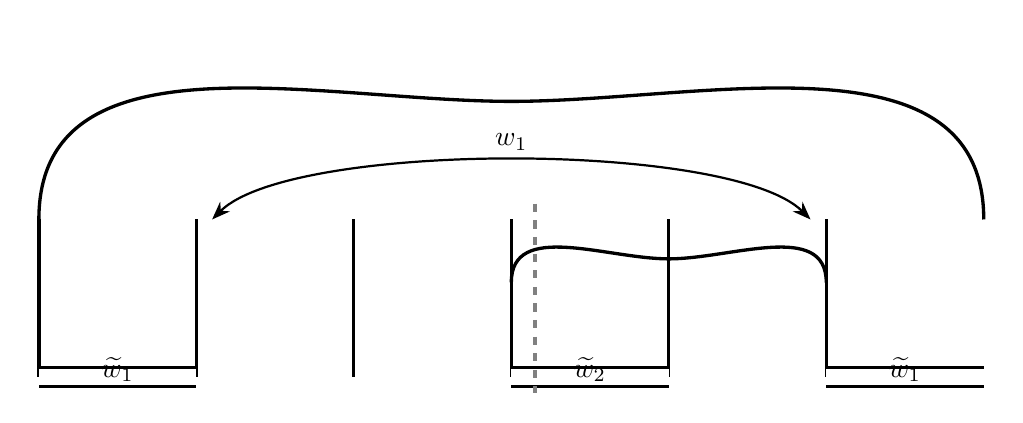
\begin{tikzpicture}[line width=1.2pt]

% Draw vertical lines
\foreach \x/\y in {0/0, 2/0, 4/0, 6/0, 8/0, 10/0}{
    \draw (\x,\y) -- (\x,\y+2);
}

% Draw horizontal bars
\draw[double distance=2mm] (0,0) -- (2,0) node[midway, above, yshift=-2mm]{$\widetilde{w}_{1}$};
\draw[double distance=2mm] (6,0) -- (8,0) node[midway, above, yshift=-2mm]{$\widetilde{w}_{2}$};
\draw[double distance=2mm] (10,0) -- (12,0) node[midway, above, yshift=-2mm]{$\widetilde{w}_{1}$};

% Draw curved arrow from left bar to right bar
\draw[->, thick, Stealth-Stealth] (2.2,2) .. controls +(1,1) and +(-1,1) .. node[above] {$w_{1}$} (9.8,2);

% Draw dashed diagonal line connecting top curve to second bar
\draw[dashed, gray] (6.3,2.2) -- (6.3,-0.2);

% Draw arc connecting first and last vertical lines
\draw (0,2) to[out=90,in=180] (6,3.5) to[out=0,in=90] (12,2);

% Draw smaller arc connecting second and third vertical lines
\draw (6,1.2) to[out=90,in=180] (8,1.5) to[out=0,in=90] (10,1.2);

\end{tikzpicture}
\end{document}